\documentclass[english,12pt,a4paper,twoside,titlepage,leqno,fleqn]{article}
\usepackage{amsmath,amssymb,amsthm,amsfonts}
\usepackage{xcolor}
\usepackage{nameref}
\usepackage{babel}
\usepackage{hyperref}
\usepackage{xparse}
\usepackage{minted}
\usepackage{graphicx}
\usepackage{savetrees}
\usepackage{tikz}

\title{Engineering Economics}
\author{Nima Poshtiban}
\date{\today}
\begin{document}

\maketitle
\tableofcontents

\section{Engineering Economics Formulas}

\subsection{Files}
\begin{itemize}
	\item \href{source}{engeco.h}
	\item \href{csource}{engeco.c}
\end{itemize}
\pagebreak
\begin{center}
\begin{table}[h]
\begin{tabular}{||c | c ||}
\hline
Symbols & Definition \\
\hline\hline
\textit{P} & 	Present Worth \\
\hline
\textit{F} & Future Worth \\
\hline
\textit{A} & Uniform Annual Amount \\
\hline
\textit{G}	& Uniform Gradient Amount \\
\hline
\textit{i} & Interest rate per interest period \\
\hline
\textit{g} & The geometric gradient \\
\hline
\textit{n} & Number of interest periods \\
\hline
\textit{m} & Number of compounding sub periods per period \\
\hline
\textit{r} & Nominal interest rate per interest period \\
\hline
\end{tabular}
\centering
\caption{Table of Symbols used in Formulas}
\end{table}
\end{center}\vspace{5cm}

\subsection{Functions}
\centering

\begin{enumerate}
	\item {\bfseries Discrete Payments }\vspace{1cm}
	\begin{enumerate}
		\item {\bfseries Discrete Compounding}\vspace{1cm}
\begin{itemize}

\item double {\bfseries calculate\_interest} \small{(double f, double p,int n)}\\
Calculates the \underline{interest}using\vspace{1cm} \[interest = \sqrt[n]{f/p}\]\vspace{1cm}

\item double {\bfseries calculate\_future} \small{(double p, double i, int n)}\\
Calculates the \underline{Future} using\vspace{1cm} \[F = P\cdot(1+i)^{n}\]
\vspace{1cm}

\item double {\bfseries calcualate\_future\_via\_annual\_uniform} \small{(double annual\_uniform, double interest, int n)}\\
Calculates the \underline{Future} using\vspace{1cm} \[F = A\cdot\left[\frac{(1+i)^{n}-1}{i}\right] \]\vspace{1cm}

\item double {\bfseries calculate\_ror } \small{(double benefit, double present)}\\
Calculates the \underline{Rate Of Return(ROR)} using\vspace{1cm} \[ROR = \frac{benefit}{P}\cdot100 \]\vspace{1cm}

\item int {\bfseries calculate\_n } \small{(double i, double f, double p)}\\
Calculates the \underline{n} using\vspace{1cm} \[n = \left\lceil\frac {\ln(\frac{F}{P})}{\ln(i+1)}\right\rceil \]\vspace{1cm}

\item double {\bfseries calculate\_present} \small{(double f, double i, double n)}\\
Calculates the \underline{Present} using\vspace{1cm} \[P = \frac{F}{(1+i)^{n}}\]\vspace{1cm}

\item double {\bfseries calculate\_summation} \small{(int start,\,int end,\,double interest,\,double annual\_uniform)}\\
Calculates the \underline{total present} using \vspace{1cm} \[P = \sum_{n=start}^{end}{A\cdot\left[\frac{1}{\left(1+i\right)^{n}}\right]}
\]\vspace{1cm}

\item double {\bfseries  calculate\_summation\_via\_geometric\_progression} \small{(double a1,\,double r,\,double annual\_uniform,\,int n)}\\
Calculates the \underline{total present summation} using\vspace{1cm} \[P_{0}=a_{1}\cdot\left(\frac{1-r^{n}}{1-r}\right)
\]\vspace{1cm}

\item double {\bfseries  calculate\_summation\_with\_gradient} \small{(double gradient, double annual\_uniform, double interest, int n)}\\
Calculates the \underline{total present summation} using\vspace{1cm} $P_{T}=P_{A}+P_{G}$\\
Example:\\
\begin{figure}[h]
	\centering
Given $P_{T}$ Chart\\
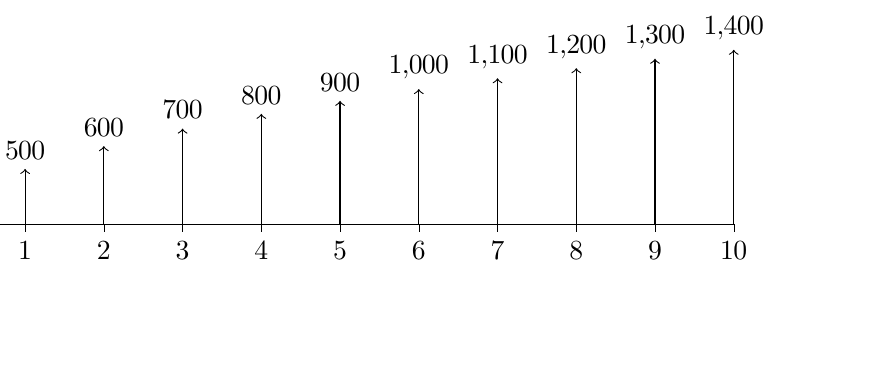
\begin{tikzpicture}[align=center]
\draw[->] (10,0) -- (0,0) -- (0,3) node[above right]{$P_{T}$};
\foreach \x in {1,...,10}{
\draw[->] (\x,0) -- (\x,{0.7*sqrt(\x)}) node[above]{\pgfmathparse{400+\x*100}\pgfmathprintnumber[    % Print the result
	fixed,
	fixed zerofill,
	precision=0
	]{\pgfmathresult}};
}
\foreach \x in {1,...,10}{
\draw[ultra thin] (\x,0) -- (\x,-0.1) node[below]{\x};
}
\end{tikzpicture}\vspace{1cm}\\
Separate it into $P_{A}$ and $P_{G}$ charts\\
\begin{tikzpicture}[align=center]
\draw[->] (10,0) -- (0,0) -- (0,3) node[above right]{$P_{A}$};
\foreach \x in {1,...,10}{
	\draw[->] (\x,0) -- (\x,0.9) ;
}
\node[above] at (5,1.3) {$A=500$};
\foreach \x in {1,...,10}{
	\draw[ultra thin] (\x,0) -- (\x,-0.1) node[below]{\x};
}
\end{tikzpicture}\vspace{1cm}\\
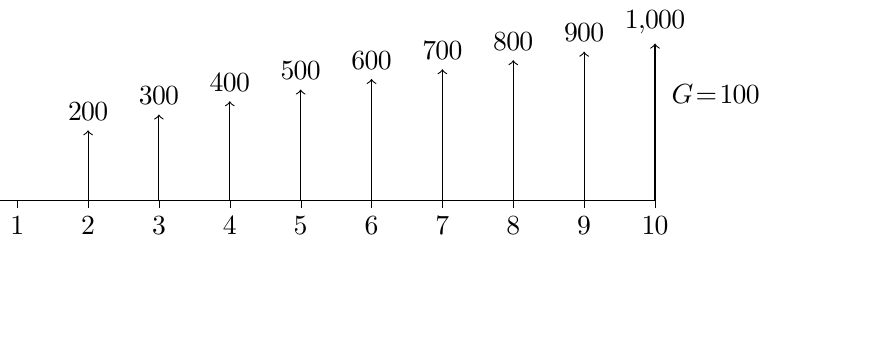
\begin{tikzpicture}[scale=0.9,align=right]
	\draw[->] (10,0) -- (0,0) -- (0,3) node[above right]{$P_{G}$};
	\foreach \x in {2,...,10}{
		\draw[->] (\x,0) -- (\x,{0.7*sqrt(\x)}) node[above]{\pgfmathparse{\x*100}\pgfmathprintnumber[    % Print the result
			fixed,
			fixed zerofill,
			precision=0
			]{\pgfmathresult}};
	}
	\node[right] at (10.1,1.5) {$G=100$};
	\foreach \x in {1,...,10}{
		\draw[ultra thin] (\x,0) -- (\x,-0.1) node[below]{\x};
	}
\end{tikzpicture}\vspace{1cm}\\

\begin{align}
	P_{T}  &= P_{A} + P_{G} \\
	P_{T}  &= P_{A}+P_{G} \\
	P_{T} &= 500\cdot\left[\frac{(1+5\%)^{10}-1}{5\%\cdot(1+5\%)^{10}}\right]+\frac{100}{5\%}\cdot\left[\frac{(1+5\%)^{10}-1}{i\cdot(1+5\%)^{10}} - \frac{10}{(1+5\%)^{10}}\right]\simeq7026.05
\end{align}
\end{figure}


\vspace{1cm}

\item double {\bfseries calculate\_present\_via\_annual\_uniform} \small{(double annual\_uniform, double interest, int n)}\\
Calculates the \underline{Present} using\vspace{1cm} \[P = A\cdot\left[\frac{(1+i)^{n}-1}{i\cdot(1+i)^{n}}\right]\]\vspace{1cm}

\item double {\bfseries calculate\_present\_via\_gradient} \small{(double gradient, double interest, int n)}\\
Calculates the \underline{Present with gradient} using\vspace{1cm} \[P = \frac{G}{i}\cdot\left[\frac{(1+i)^{n}-1}{i\cdot(1+i)^{n}} - \frac{n}{(1+i)^{n}}\right]\]\vspace{1cm}

\item double {\bfseries calculate\_present\_via\_geometric\_gradient} \small{(double a1, double i, double g, int n)}\\
Calculates the \underline{Present with geomatric gradient} using\vspace{1cm} \[P = A_{1}\cdot\left[\frac{1-(1+g)^{n}\cdot(1+i)^{-n}}{i-g}\right]\] Where $i\neq g$\vspace{1cm}


\item double {\bfseries calculate\_annual\_uniform\_via\_present} \small{(double present, double interest, int n)}\\
Calculates the \underline{Annual Uniform} using\vspace{1cm} \[A = P\cdot\left[\frac{i\cdot(1+i)^{n}}{(1+i)^{n}-1}\right]\]\vspace{1cm}

\item double {\bfseries calculate\_annual\_uniform\_via\_future} \small{(double future, double interest, int n)}\\
Calculates the \underline{Annual Uniform} using\vspace{1cm} \[A = F\cdot\left[\frac{i}{(1+i)^{n}-1}\right]\]\vspace{1cm}

\item double {\bfseries calculate\_annual\_uniform\_via\_gradient} \small{(double gradient, double interest, int n)}\\
Calculates the \underline{Annual Uniform} using\vspace{1cm} \[A = G\cdot\left[\frac{1}{i}-\frac{n}{(1+i)^{n}-1}\right]\]\vspace{1cm}

\item double {\bfseries calculate\_effective\_interest\_rate} \small{(double r, double m)}\\
Calculates the \underline{Effective Interest Rate} using\vspace{1cm} \[i_{eff}=(1+\frac{r}{m})^{m}-1\]\vspace{1cm}
\end{itemize}
\item {\bfseries Continuous Compounding}\vspace{1cm}
\begin{itemize}
	\item double {\bfseries calculate\_future\_c} \small{(double p, double r, int n)}\\
	Calculates the \underline{Future} using\vspace{1cm} \[F = P\cdot(e)^{r\cdot n}\]
	\vspace{1cm}
	\item double {\bfseries calculate\_present\_c} \small{(double f, double r, int n)}\\
	Calculates the \underline{Present Worth} using\vspace{1cm} \[P = \frac{F}{(e)^{r\cdot n}}\]
	\vspace{1cm}
	\item double {\bfseries calcualate\_future\_via\_annual\_uniform\_c} \small{(double annual\_uniform, double r, int n)}\\
	Calculates the \underline{Future} using\vspace{1cm} \[F = A\cdot\left[\frac{(e)^{r\cdot n}-1}{e^{r}-1}\right] \]\vspace{1cm}

	\item double {\bfseries calculate\_present\_via\_annual\_uniform\_c} \small{(double annual\_uniform, double r, int n)}\\
	Calculates the \underline{Present} using\vspace{1cm} \[P = A\cdot\left[\frac{e^{r\cdot n}-1}{e^{r\cdot n}\cdot e^{r}-1}\right]\]\vspace{1cm}

	\item double {\bfseries calculate\_annual\_uniform\_via\_present\_c} \small{(double present, double r, int n)}\\
	Calculates the \underline{Annual Uniform} using\vspace{1cm} \[A = P\cdot\left[\frac{ e^{r\cdot n}\cdot (e^{r}-1)}{e^{r\cdot n}-1}\right]\]\vspace{1cm}

	\item double {\bfseries calculate\_annual\_uniform\_via\_future\_c} \small{(double future, double r, int n)}\\
	Calculates the \underline{Annual Uniform} using\vspace{1cm} \[A = F\cdot\left[\frac{e^{r}-1}{e^{r\cdot n}-1}\right]\]\vspace{1cm}

%	\item double {\bfseries calculate\_annual\_uniform\_via\_gradient\_c} \small{(double gradient, double r, int n)}\\
%	Calculates the \underline{Annual Uniform} using\vspace{1cm} \[A = G\cdot\left[\frac{1}{e^{r}-1}-\frac{n}{(e)^{r\cdot n}-1}\right]\]\vspace{1cm}

	\item double {\bfseries calculate\_effective\_interest\_rate\_c} \small{(double r)}\\
	Calculates the \underline{Effective Interest Rate} using\vspace{1cm} \[i_{eff}=e^{r}-1\]\vspace{1cm}
\end{itemize}
\end{enumerate}
\item {\bfseries Continuous Payments }\vspace{1cm}
\begin{itemize}
	\item double {\bfseries calculate\_future\_c} \small{(double p, double r, int n)}\\
	Calculates the \underline{Future} using\vspace{1cm} \[F = P\cdot(e)^{r\cdot n}\]
	\vspace{1cm}
	\item double {\bfseries calculate\_present\_c} \small{(double f, double r, int n)}\\
	Calculates the \underline{Present Worth} using\vspace{1cm} \[P = \frac{F}{(e)^{r\cdot n}}\]
	\vspace{1cm}
\end{itemize}
\end{enumerate}

\section{Source Code}
\subsection{engeco.h}\label{source}
%\inputminted[linenos]{c}{./engeco.h}
\subsection{engeco.c}\label{csource}
%\inputminted[linenos]{c}{./engeco.c}
\end{document}